\documentclass[a4paper,12pt]{book}

\usepackage[font=scriptsize]{caption}
\usepackage[T1]{fontenc}
\usepackage[italian,english]{babel}
\usepackage[utf8]{inputenc}
\usepackage{graphicx}
\usepackage{color}
\usepackage{cite}
\usepackage{amsmath}
\usepackage{amssymb}
\usepackage{amsthm}
\usepackage{wasysym}
\usepackage{setspace}
\usepackage{algorithm}
\usepackage{algorithmic}
\usepackage{multirow}
\usepackage{listings}
\usepackage{url}
\usepackage[height=21.6cm,width=15cm,centering]{geometry}

\usepackage[bookmarks=true,hyperindex,colorlinks=false,
            pdfborder={0 0 0},pdfstartview=FitH,pdfpagelayout=SinglePage,
            pdfauthor={Marco Edemanti},
            pdftitle={TITOLO},
            pdfsubject={}]{hyperref}

\title{RASD WeatherCal}
\author{Edemanti Marco}
\author{Polidori Paolo}

\begin{document}
\selectlanguage{english}
\lstset{ %
  backgroundcolor=\color{white},   % choose the background color; you must add \usepackage{color} or \usepackage{xcolor}
  basicstyle=\footnotesize,        % the size of the fonts that are used for the code
  breakatwhitespace=false,         % sets if automatic breaks should only happen at whitespace
  breaklines=true,                 % sets automatic line breaking
  captionpos=b,                    % sets the caption-position to bottom
  commentstyle=\color{green},    % comment style
  deletekeywords={...},            % if you want to delete keywords from the given language
  escapeinside={\%*}{*)},          % if you want to add LaTeX within your code
  extendedchars=true,              % lets you use non-ASCII characters; for 8-bits encodings only, does not work with UTF-8
  frame=single,                    % adds a frame around the code
  keepspaces=true,                 % keeps spaces in text, useful for keeping indentation of code (possibly needs columns=flexible)
  keywordstyle=\color{blue},       % keyword style
  language=Java,                 % the language of the code
  morekeywords={*,...},            % if you want to add more keywords to the set
  numbers=left,                    % where to put the line-numbers; possible values are (none, left, right)
  numbersep=5pt,                   % how far the line-numbers are from the code
  showspaces=false,                % show spaces everywhere adding particular underscores; it overrides 'showstringspaces'
  showstringspaces=false,          % underline spaces within strings only
  showtabs=false,                  % show tabs within strings adding particular underscores
  stepnumber=2,                    % the step between two line-numbers. If it's 1, each line will be numbered
  tabsize=2,                       % sets default tabsize to 2 spaces
}
 \begin{center}
    
\includegraphics[width=4cm]{immagini/polilogo.png}
    \end{center}
\begin{center}

{\huge{\bf\uppercase {Requirements Analysis  \\and \vspace*{0.5cm} \\Specification Documents}}}


\end{center}
\vspace*{0.5cm}
\begin{center}
{\large Project of Software Engineering 2\\ \vspace*{0.5cm} \huge WEATHER-CAL}
\end{center}
\begin{flushright}
 \vspace*{9cm}

        {\bf Authors: }\\
        \vspace*{0.2cm}
            {\bf   {PAOLO POLIDORI} }\\
             \vspace*{0.3cm}
            {\bf   {MARCO EDEMANTI} }
    \end{flushright}

\doublespacing    
\tableofcontents
\listoffigures


\chapter{Introduction} \label{cap:cap1}

\section{Purpose}
The purpose of this document is to present a description of WheaterCal system. It will explain the features of the system, the interfaces of the system, what the system will do and the constraints under which it must operate.
This document is intended for both the stakeholders and the developers of the system.
Stakeholders of the system are the client, which is our teacher and their assistants, composing the group that will evaluate our project, the testers, which are a team with our same project and our same tasks and the developers, which are the authors of this document.

\section{Scope}
We want to project and implement WheaterCal. The aim of this project is to develop a system that offers an online calendar in which user can schedule their events according to the weather conditions.\\ A registered user can create, delete and update an event and moreover he should provide information about where and when this event will take place and information about the invited user.
Once the event is created the system should provide to its creator the weather forecast information regarding the scheduled day, and most of all it should notify a bad weather condition one day in advance to all the participants.\\
Also a user is able to make his/her calendar visible to all other registered user showing them only the time slots in which they are busy without letting know the event information unless either the event is public.
In addition in case of bad weather, three day before the scheduled data of an event, the system will inform the event's owner and propose to him the closest sunny day.

\section{Glossary}
\begin{tabularx}{\linewidth}{|r|X|}
  \hline  {\bf Anonymous User} & People who access the system but didn't authenticate\\ 
  \hline  {\bf Registered User} & People who both registered to the platform and logged in. Sometimes referred to as "User"\\ 
  \hline  {\bf Platform, System} & The WeatherCal application\\
  \hline  {\bf Bad Weather}&  Undesired conditions for an event to take place basing on the event owner's choices\\
  \hline  {\bf Notification} & A message that arrives to the user in dedicated area, which can be easily identified by the user at first sight\\
  \hline  {\bf Event owner} & The user who created the event and for which is responsibile of the organization\\
  \hline  {\bf Event invited} & A user invited to an event for which can decide if he wants to be a participant or not\\
  \hline  {\bf Event participant} & A user invited to an event for which decided to participate\\
  \hline  {\bf Event} & An occurrence, which was inserted in the system which should happen in a certain date and a certain time\\
  \hline  {\bf Calendar} & The set of all the events for a user, shown in a per-month view\\
  \hline
\end{tabularx}\\
\section{References}
IEEE,{\it IEEE Std 830-1998,IEEE Recommended Practice for Software Requirements Specifications},  IEEE Computer Society 1998

 
\chapter{Overall Description} \label{cap:cap2}
\section{System Environment}
WeatherCal is a stand alone software made from scratch. It is a Web application that allows the registered users to manage their schedule basing on the weather conditions. The users are also able to invite people to their event and to publicize their event.  
The system is even capable of notifying the users, as they log on to the system, if the weather forecast for the event is not the desired one.
The target of this software is, therefore, to give the users a tool for schedule their events smartly, giving the possibility to change preferences as the weather forecast changes.
\subsection{Actors}
Actors in the system are mainly the people registered into the web application. They will be referred as Registered Users.
Whoever is not yet registered on the platform will be an actor for the system too and it will be identified as an Anonymous  Users.
No administration is required since the system is not intended for illicit purposes and this is a policy of the platform, plus no conflict among users can occur since the only allowed interactions are the invite to an event and a participation to an event (in which other people partecipate).
\subsection{Scenarios}
\begin{itemize}
\item Maggie creates an event for her daughter's birthday, which will be in their garden. She invites all her friends telling them to join the event on WeatherCal to be sure that the forecast will be graceful for that day. Three days before the birthday, Maggie logs in two days before the event and she discovers it will be cloud but she still hopes it won't rain on that day. The day before the event Judith, Maggie's friend, is notified that it could be rainy for the birthday as she logs into the system. Anyway Maggie decides she won't posticipate the birthday. In the end that day was rainy, except for the afternoon, exactly for the birthday, and everything went fine.
\item John wants to go cycling but right now the forecast is not so optimistic, so he decides to use WeatherCal to find the best day for doing so. The platform suggests him that he should go on Monday afternoon, so he plans to do that. Saturday he logs in and discovers that it will be windy on Monday, infact the system suggests him to go cycling on Wednesday and John chooses to do what the system suggests him. In the end he went cycling and the weather was perfect.
\item Beth wants to have a picnic with her friends in two weeks, so she creates an event on WeatherCal when the temperature should be the hottest and there should be no clouds in the sky. Three days before she logs in discovering that for the next two weeks there will be bad weather conditions. She decides so to invite her friends at home for having a launch together.
\end{itemize}
\section{Functional Requirements}
The system allows the users to partecipate in various scenarios:
\begin{itemize}
\item Log on to and log out from the platform.
\item Create, Modify, Delete an event.
\item Invite other users.
\item Manage participations (accept, refuse, ...).
\item Manage event visibility (decide if an event's infos should be accessible only by its invited). 
\item View other users' profiles (see other users's calendar only if it's set public and see the events' details if they mark public too or you are invited to them)
\end{itemize}
The system is the leading actor in:
\begin{itemize}
\item {Warning all the participants to an event which will occur the following day that there will be bad weather conditions if so.} 
\item Notify to an event's owner three day before the scheduled data that there will be bad conditions for it suggesting the closest available sunny day.
\end{itemize}
The Anonymous Users are only able to:
\begin{itemize}
\item Sign Up in to the Platform.
\end{itemize}
\section {Goals}
The WeatherCal system should offer and fulfill these main features:
\begin{itemize}
\item A simple management for the users' agendas
\item A swift way to schedule an event according to the weather forecast 
\item Invite other registered users to an event
\item Preserve the privacy of the users since only the user himself can make their info visibile to everyone.
\end{itemize}
\section{Non Functional Requirements}
\subsection{User Interfaces}
The WeatherCal system is a Web application intended to be used trough a desktop device.  Its interface is designed in a simple way so that  the user can either easily understand what the system can offer to him and reache all the main features of the system from a unique view.\\
Once that a user logs in to the system trough a defined web page he is redirected to the main page. This page is divided in two portions. The left one, which occupies the largest portion of the page, displays a monthly calendar in which the user manages its events while the right one shows the weather forecast for the following days and also shows the closest events.\\In the figure~\ref{fig:mockup} is shown a first sketch of the main user's page.\\ \\  
 \begin{center}
 \begin{figure}
    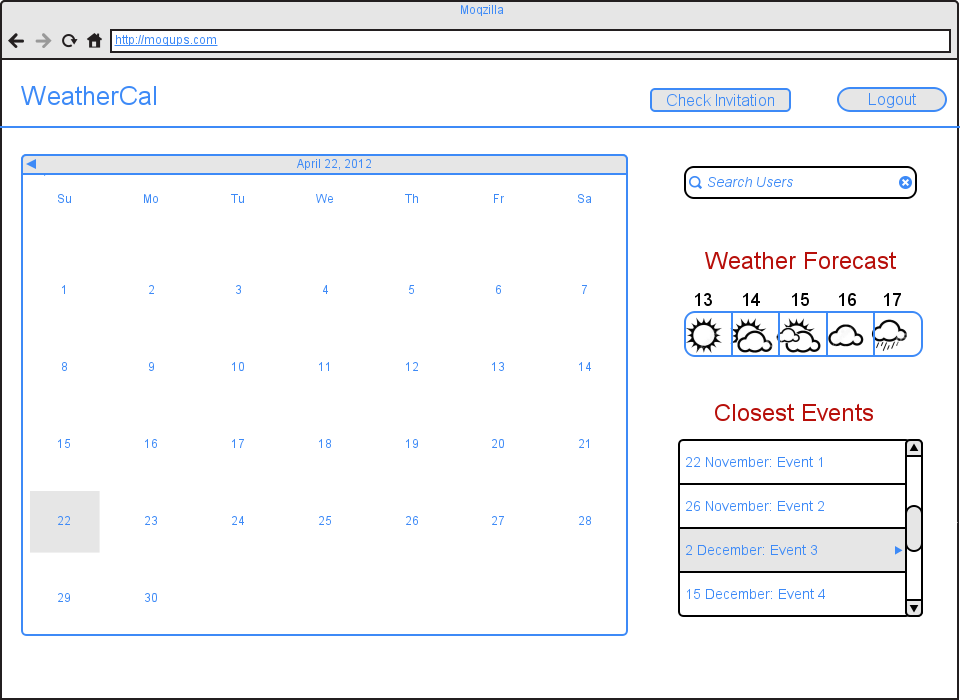
\includegraphics[width=0.9\textwidth]{immagini/UserPage.png}
    \caption{Main Page's MockUp}
     \label{fig:mockup}
     \end{figure}
    \end{center}
\subsection{Performance}
The system offers the users the possibility to use it without major slowdowns. Multiuser usage is allowed and it can be bore by the server application under reasonable conditions, basing on the server hardware.
\subsection{Security}
The system relies on HTTP protocol for transferring data over the Internet, so information sent both from the user to the server and vice-versa will be exposed to possible man-in-the-middle attacks. Unless this issue data stored on the server will be accessible only if valid credentials are provided and there is no possibility for a user to bypass privacy constraints, i.e. users will not be able to see non-public events of other users and modify events for which they are not owners. This will be accomplished from the server by performing checks on the data requested by the client (authorization politics).
\chapter{Requirement Specification} \label{cap:cap3}
\section{External Interface Requirement}
\section{Functional Requirements}
\section{Non Functional Requirements}


\end{document}
